\begin{frame}\frametitle{Requirements for Selection of $W\gamma$ Candidates}
% ADD A PLOT WITH GEOMETRY (eta)
  \begin{table}[h]
     \tiny
     \begin{center}
     \begin{tabular}{|c|c|l|}
     \hline
     \multicolumn{2}{|c|}{\scriptsize{Selection requirements for candidates}} & {\scriptsize{Comment}} \\ 
     {\bfseries{- - - - - - $W\gamma\rightarrow\mu\nu\gamma$ - - - - - -}} & 
     {\bfseries{- - - - - - $W\gamma\rightarrow e\nu\gamma$ - - - - - -}}  & \\ \hline

    \multicolumn{2}{|c|}{\scriptsize\bfseries\color{blue}{Event level selection criteria:}}  & \\ 
     \multicolumn{2}{|c|}{Exactly one lepton + at least one photon}  & process signature\\  
      \multicolumn{2}{|c|}{$M_T^W>$40~GeV} & rejects DY+jets, $Z\gamma$\\ 
                                & 110$>M_{e\gamma}>$70~GeV excl. & rejects DY+jets\\ 
      \multicolumn{2}{|c|}{$\Delta{R}(lep,\gamma)>$0.7} & theory consideration\\  \hline

     \multicolumn{2}{|c|}{\scriptsize\bfseries\color{blue}{Photon selection:}} & \\
     \multicolumn{2}{|c|}{\tiny{$P_T^{\gamma}>$15~GeV}} & theory considerations \\ 
     \multicolumn{2}{|c|}{\tiny{$\eta^{\gamma}$: EB or EE}} & acceptance \\ 
     \multicolumn{2}{|c|}{\tiny{Photon ID*}} & POG**-recommended \\ 
             &{\tiny{ [one change in ID]}} & $W\gamma\gamma$-recommended\\ \hline

     \multicolumn{2}{|c|}{\scriptsize\bfseries\color{blue}{Lepton selection:}} & \\
      \tiny{$p_T^{\mu}>$25~GeV;} &  \tiny{$p_T^{e}>$30~GeV;}  & trigger\\ 
      \tiny{$|\eta^{\mu}|<2.1$} & \tiny{  $\eta^{e}$: EB or EE} & trigger, acceptance\\ 
      Muon ID & Electron ID & POG-recommended \\ \hline

      \multicolumn{2}{|c|}{\scriptsize\bfseries\color{blue}{Second lepton veto:}} & rejects DY+jets, $Z\gamma$\\
      \tiny{$p_T^{\mu2}>10$ GeV;} &  \tiny{$p_T^{e2}>10$ GeV;} & \\
      \tiny{$|\eta^{\mu2}|<2.4$}  &   \tiny{ $\eta^{e2}$: EB or EE} &  \\
                                &   \tiny{[veto] ID} & very loose \\ \hline
      \end{tabular}
      \end{center}
  \end{table}
\scriptsize
If we have several candidates in an event, we choose one with the highest $P_T^{\gamma}$\\
\tiny
* ID - identification criteria\\
** POG - Particle Object Group (in CMS)\\
\end{frame}%{Event-Level Selection Requirements}

\begin{frame}\frametitle{$P_T^{\gamma}$ Spectrum of $W\gamma\rightarrow\mu\nu\gamma$ Candidates}
  \begin{figure}[htb]
    \begin{center}
       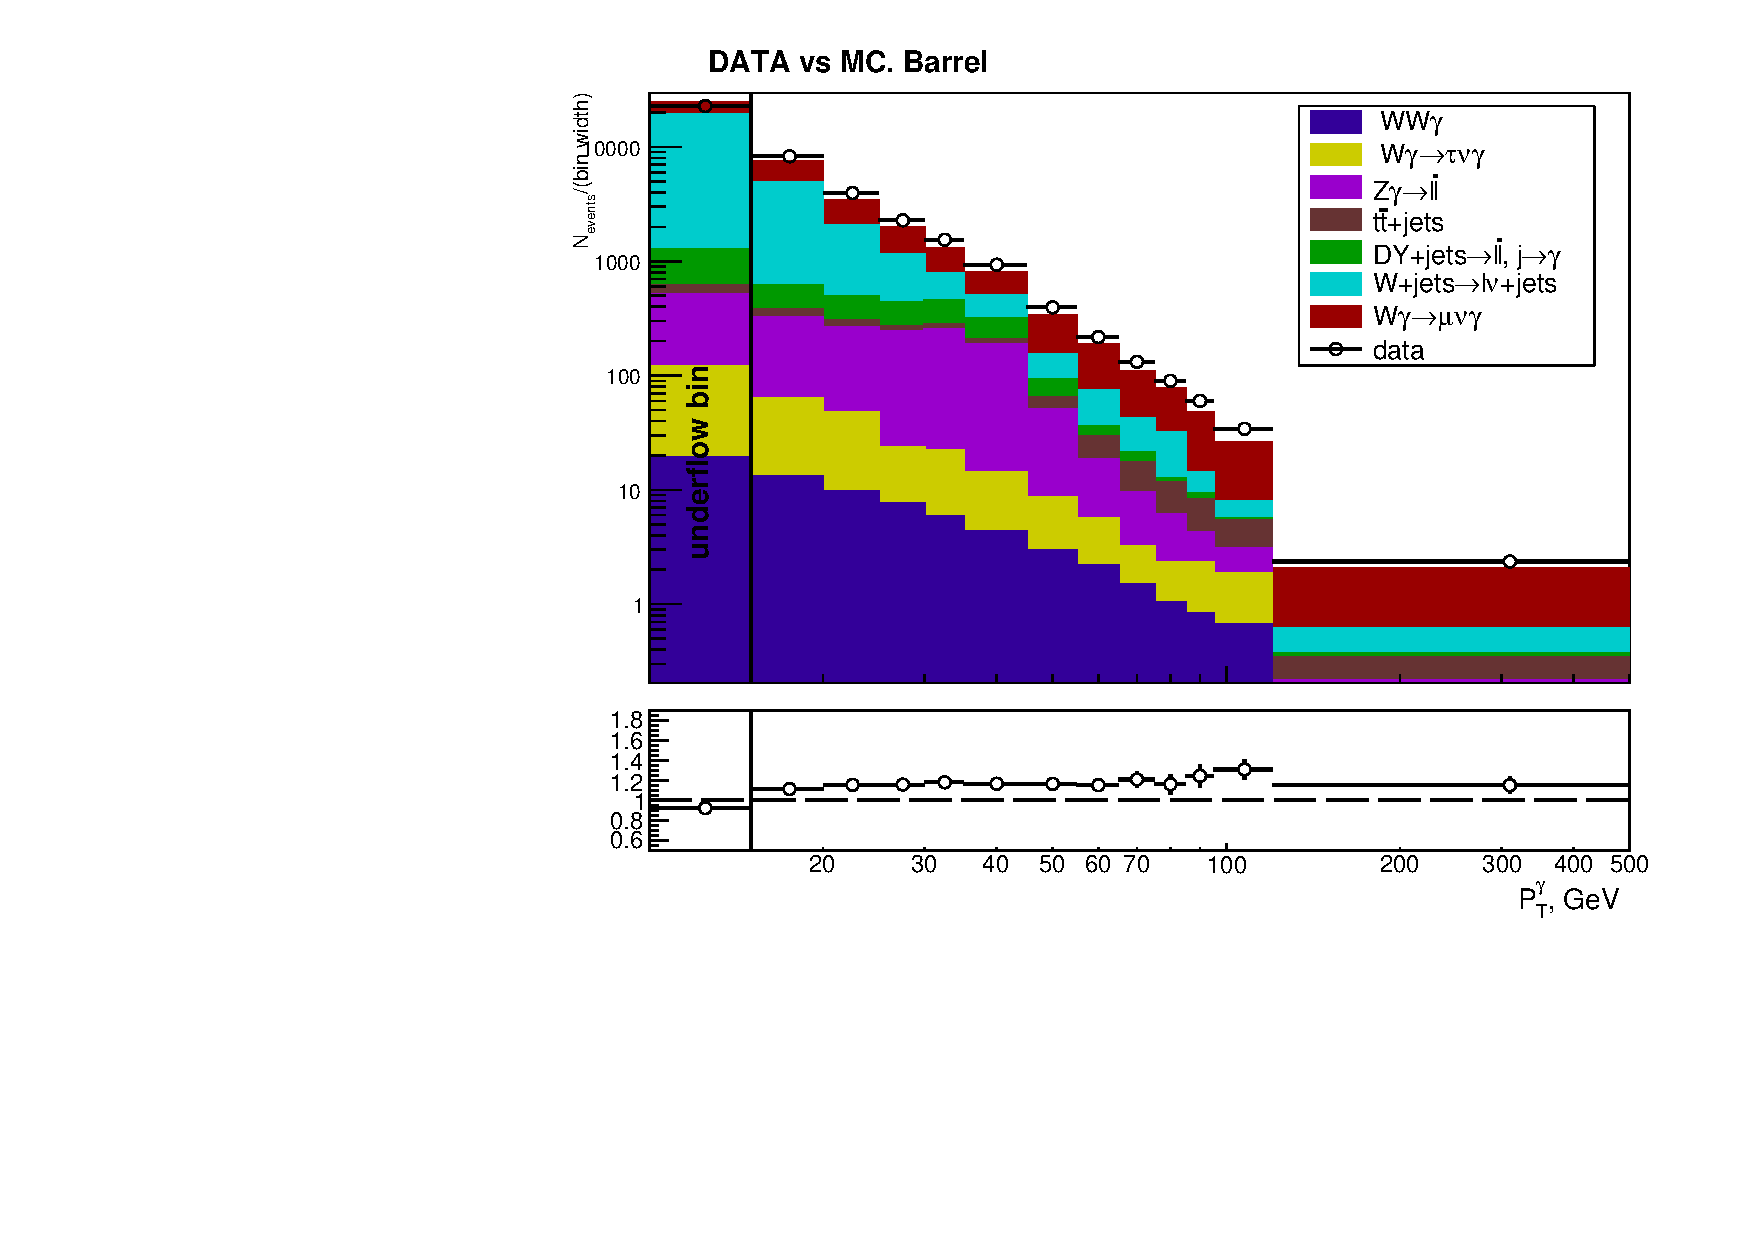
\includegraphics[width=0.65\textwidth]{../figs/figs_v11/MUON_WGamma/PrepareYields/c_TotalDATAvsMC_Barrel__phoEt.pdf}  
    \end{center}
  \end{figure}

\tiny
  \begin{table}[h]
     \tiny
     \begin{center}
     \begin{tabular}{|l|l|}
     \hline
     Dominated by $W$+jets* events in low $P_T^{\gamma}$ bins; &  {\bfseries{ Backgrounds:}}\\ 
     Fraction of signal increases with $P_T^{\gamma}$; & Jets$\rightarrow\gamma$: $W$+jets, DY+jets**, $t\bar{t}$+jets;\\
     Data disagree with MC. & Real-$\gamma$: $Z\gamma$, $W\gamma\rightarrow\tau\nu\gamma$.\\
     \hline
      \end{tabular}
      \end{center}
  \end{table}

* jets are hadronic jets (explained more later)\\
** DY+jets is Drell-Yan+jets process, can be understood as $Z$+jets

\end{frame}


